\documentclass[10pt,a4paper,twocolumn,twoside]{article}
\usepackage[utf8]{inputenc}
\usepackage[catalan]{babel}
\usepackage{multicol}
\usepackage{graphicx}
\usepackage{fancyhdr}
\usepackage{times}
\usepackage{amsmath}
\usepackage{titlesec}
\usepackage{hyperref}
\usepackage{multirow}
\usepackage{float}
\usepackage{subcaption}
\usepackage{wrapfig}
\usepackage[top=2.5cm, bottom=1.3cm, left=1.2cm, right=1.2cm]{geometry}
\usepackage[figurename=Fig.,tablename=Taula,font={small,sf}]{caption}
%\usepackage[font={small,sf}]{caption}
\hypersetup{
	pdfborder={0 0 0} 
}
\usepackage{enumitem}
\setlist[itemize]{noitemsep}
\setlist[enumerate]{noitemsep}
\usepackage[most]{tcolorbox}

\let\OLDthebibliography\thebibliography
\renewcommand\thebibliography[1]{
  \OLDthebibliography{#1}
  \setlength{\parskip}{0pt}
  \setlength{\itemsep}{0pt plus 0.3ex}
}

\pagestyle{fancy}
\fancyhf{}
\fancyhead[LO]{\textsf{\small $\mu$Projecte VC(GEI)-PSIV(GED), Escola d’Enginyeria (EE), Universitat Autònoma de Barcelona (UAB)}}
\fancyhead[RE]{\textsf{\small $\mu$Projecte VC(GEI)-PSIV(GED), Escola d’Enginyeria (EE), Universitat Autònoma de Barcelona (UAB)}}
\renewcommand{\headrulewidth}{0pt}

\titleformat*{\section}{\large\sffamily\scshape\bfseries}
\titleformat*{\subsection}{\normalsize\sffamily\bfseries}
\titleformat*{\subsubsection}{\normalsize\sffamily\slshape}

\begin{document}

{\sffamily
% Titol
\noindent\textbf{\LARGE ZebrAI Crossing: Detecció de passos de zebra i semàfors de vianants}
% autors
\begin{center}
Albert Capdevila Estadella (1587933), Levon Kesoyan Galstyan (1668018), Luis Martínez Zamora (1668180)
\end{center}

%\bigskip
\bigskip

\noindent 
\textbf{Abstract} --- Lorem ipsum dolor sit amet, consectetur adipiscing elit. In auctor est et lacus luctus eleifend. Duis at tincidunt nibh. Nam sed elementum lorem, eu pretium magna. Vestibulum justo urna, imperdiet eget tristique ut, pellentesque vel turp-is. Vivamus et risus tempor, fringilla libero in, semper arcu. Praesent blandit libero vitae rutrum tincidunt. Fusce id justo quis mauris accumsan pellentesque et in massa. Nulla ut eleifend ante. Nunc pretium justo a nibh tincidunt tempus. Fusce auctor tortor nec turpis commodo, vitae posuere nulla mollis. Maecenas non placerat metus. Mauris dolor libero, laoreet quis leo vitae, dignissim lobortis enim. Curabitur in magna nibh. Aenean vel dui eros. Morbi maximus in turpis vitae fermentum.

\bigskip

\noindent 
\textbf{Keywords}---Image classification, noisy web data, CNNs, ubiquitous reweighting.
}
\bigskip

{\vrule depth 0pt height 0.5pt width 3cm\hspace{7.5pt}%
\raisebox{-3.5pt}{\fontfamily{pzd}\fontencoding{U}\fontseries{m}\fontshape{n}\fontsize{11}{12}\selectfont\char70}%
\hspace{7.5pt}\vrule depth 0pt height 0.5pt width 3cm\relax}

%\bigskip


\section{Introducció}

\textbf{ZebrAI Crossing} és un model de visió per computador que, donada una imatge en un entorn urbà, detecta si hi apareix un pas de zebra i en determina la seva orientació i posició respecte la càmera. A més a més, també detecta la presència de semàfors per a vianants i indica el seu estat (en vermell, en verd...).

\subsection{Objectius}
\vspace{-0.3em}
\begin{itemize}
	\item Identificar si apareix un pas de zebra a la imatge.
	
	\vspace{0.3em}
	\textit{En cas afirmatiu:}
	\begin{itemize}[label=\textbullet]
		\item {Determinar l’orientació del pas de zebra.}
		\item {Determinar la posició de l'inici del pas de zebra.}
	\end{itemize}
	\item {Identificar si apareix un semàfor de vianants a la imatge.}
	
	\vspace{0.3em}
	\textit{En cas afirmatiu:}
	\begin{itemize}[label=\textbullet]
		\item {Indicar si el semàfor es troba en verd.}
	\end{itemize}
\end{itemize}

\section{Estat de l'art}
Aquests són els recursos que ens han resultat més útils de tots els que hem investigat (Veure \hyperref[sec:biblio]{Referències}):

\subsection{Projectes}\label{sec:projectes}
\subsection*{ImVisible \cite{ImVisible}}
El projecte tracta del desenvolupament d'una aplicació mòbil que detecta passos de zebra, la seva orientació i, si hi ha semàfor, identifica si està en verd o vermell. Tot el procés de reconeixement d'imatges es fa mitjançant xarxes neuronals convolucionals. L'aspecte que ens ha sigut més útil és el \textbf{dataset} que utilitza, anomenat Pedestrian Traffic Lights, perquè té moltes imatges anotades amb atributs que ens interessen.

\subsection{Articles}\label{sec:articles}
\subsection*{Zebra-crossing Detection for the Partially Sighted \cite{ZebraPartiallySighted}}
Aquest article utilitza transformacions de Hough i detecció de variacions d'intensitat per a identificar les línies defineixen el pas de zebra. A més, es proven diferents mètodes per diferenciar-los d'imatges d'escales, un basat en homografies i els altres amb restriccions basades en els punts de fuga.

\subsection*{ZebraRecognizer: efficient and precise localization of pedestrian crossings. \cite{ZebraRecognizer}}

Aquest article explica un mètode que combina la càmera amb l’acceleròmetre del mòbil de l'usuari per rectificar la perspectiva abans de detectar els passos de zebra. Una vegada rectificada, l’algorisme detecta els segments amb EDLines i els valida segons solapament i consistència de color. Els autors reporten molts bons resultats, però no els hem pogut replicar perquè la rectificació amb sensors inercials no és aplicable al nostre projecte.

\subsection*{Zebra-crossing detection based on cascaded Hough transform principle and vanishing point characteristics \cite{CascadedHough}}

L'article presenta un estudi per detectar passos de zebra utilitzant un filtratge de Gauss, detecció de vores de Canny i una transformada en cascada de Hough basada en el punt de fuga, sense extreure regions d'interès. També es compara amb la transformada de Hough estàndard, demostrant que la tècnica en cascada obté millors resultats.

\subsection*{ZebraRecognizer: Pedestrian crossing recognition for people with visual impairment or blindness \cite{RobustPedestrian}}
Aquest article presenta una app per invidents que detecta passos de zebra en temps real mitjançant una homografia per corregir la perspectiva, sobre la qual aplica una detecció de vores. Finalment, utilitza regressió ortogonal per identificar una línia comuna entre els segments detectats.

\section{Proposta}

\subsection{Descripció de les dades}
En aquest projecte, hem utilitzat un conjunt de dades fabricat a partir de dos datasets diferents: \textbf{Pedestrian Traffic Lights \cite{ImVisible}} i \textbf{GlobalStreetscapes \cite{GlobalStreetscapes}}.
Aquest conjunt de dades s’ha utilitzat per avaluar i provar la detecció de passos de zebra i els seus atributs, així com per provar la detecció de l’estat dels semàfors per a vianants.

\textbf{Pedestrian Traffic Lights} proporciona una gran quantitat d'imatges anotades amb l'estat del semàfor de vianants i dos punts que defineixen un segment perpendicular al pas de zebra.
Així doncs, hem extret la orientació del pas de zebra i la posició de l'inici d'aquest amb els càlculs:
\begin{equation*}
	\theta = \tan^{-1}\left( \frac{x_2 - x_1}{y_2 - y_1} \right) \ \ \quad
	(x, y) = (x_i, y_i : y_i > y_{3-i})
\end{equation*}
A més, per a fer una bona avaluació, ha sigut necessari afegir imatges que no continguin passos de zebra, motiu pel qual hem decidit incorporar imatges de \textbf{GlobalStreetscapes}.

Per tant, els atributs finals que té cada imatge del dataset que hem construït són: \textbf{\texttt{[file, zebra, mode, blocked, x, y, theta\_rad, theta\_deg]}}, on \texttt{zebra} indica si hi ha pas de zebra o no, \texttt{mode} indica l'estat del semàfor, \texttt{blocked} indica si el semàfor no és visible (bloquejat), (\texttt{x}, \texttt{y}) és la posició de l'inici del pas de vianants i \texttt{theta} és l'angle entre la línia de creuament i l’eix vertical de la imatge (eix y). És a dir, la càmera hauria de girar $\theta$º per poder creuar el pas de zebra avançant cap endavant.\footnote{És una simplificació que no té en compte la distorsió provocada pels punts de fuga. Les rectes paral·leles a la realitat no sempre ho són a la imatge, pel que el gir desitjat no és exactament $\theta$º}

\subsection{Tècniques a utilitzar}
 
 Aquest projecte combina dues metodologies: \textbf{tècniques tradicionals} per a detectar els passos de zebra i els seus atributs, com ara morfologia matemàtica, detecció de vores,... i \textbf{tècniques basades en deep learning} per a la detecció dels semàfors i el seu estat, amb eines com ara YOLO \cite{YOLO}.
 
\section{Experiments, resultats i anàlisi}
%\begin{figure}[!h]
%	\centering
%	\includegraphics[width=0.95\linewidth]{figs/filtratge}
%	\caption{Angle d'orientació del pas de zebra}
%	\label{fig:f}
%\end{figure}

\subsection{Extracció dels atributs del pas de zebra}

En aquest apartat hem usat la ROI prèvia per determinar l’orientació i la posició inicial del pas de zebra. Ho hem fet identificant-ne primer les vores paral·leles.

Les imatges amb les que hem treballat tenien molt \textbf{soroll impulsional}, i a més, normalment la pintura dels passos de zebra presenta molts desperfectes, pel que hem hagut d'aplicar un filtratge de soroll. N'hem provat quatre: mediana, Gaussià, bilateral (similar al Gaussià però mantenint millor les vores) i morfologia de màxims (dilate, per omplir forats a la pintura).
\begin{figure}[!h]
	\centering
	\begin{subfigure}{0.46\columnwidth}
		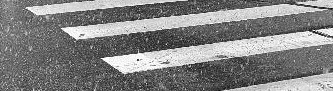
\includegraphics[width=\linewidth]{figs/neu1}
		\caption{Imatge original}
	\end{subfigure}
	\quad
	\begin{subfigure}{0.46\columnwidth}
		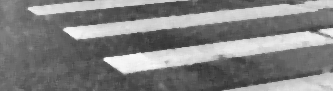
\includegraphics[width=\linewidth]{figs/med_neu1}
		\caption{Filtre de mediana}
	\end{subfigure}
	\caption{Exemple del filtratge de soroll}
	\label{fig:soroll}
\end{figure}
\\
El \textbf{filtre de mediana} ha donat un bon resultat visual: les barres del pas de zebra es veuen nítides i, en casos com el de la Figura.~\ref{fig:soroll}, on plou, elimina tot el soroll de la pluja, a diferència de les altres opcions.

Una vegada hem tingut la imatge filtrada, hem decidit treure'n una màscara binària per detectar-ne millor les vores.
\vspace*{0.5em}
\\
{\small	\textbf{El problema del top-hat:}}\vspace*{0.2em}\\
En algunes imatges, les ombres han dificultat l’extracció de la màscara binària. La tècnica del \textbf{top-hat} és útil en situacions així, però ens hem trobat amb un problema: no hi ha un kernel que funcioni bé ni per a totes les imatges ni dins la mateixa imatge, ja que la mida i orientació de les barres varia amb la perspectiva. Un kernel petit només destaca les barres llunyanes, i un de gran no elimina les ombres. Així doncs, en aquests casos la precisió dependrà de les parts menys afectades per les ombres.
\vspace*{0.5em}
\\
Totes les imatges són diferents, motiu pel qual aplicar un llindar constant a totes elles no era una opció viable. Hem utilitzat el llindar adaptatiu \textbf{Otsu}, implementat en la funció d'\texttt{OpenCV}. Ara bé, analitzant l'histograma d'algunes de les imatges, hem vist que l'Otsu no segueix la nostra intuició d'un millor llindar: situar-lo a la vall entre els pics dels clars i els foscos.
\begin{figure}[!h]
	\centering
	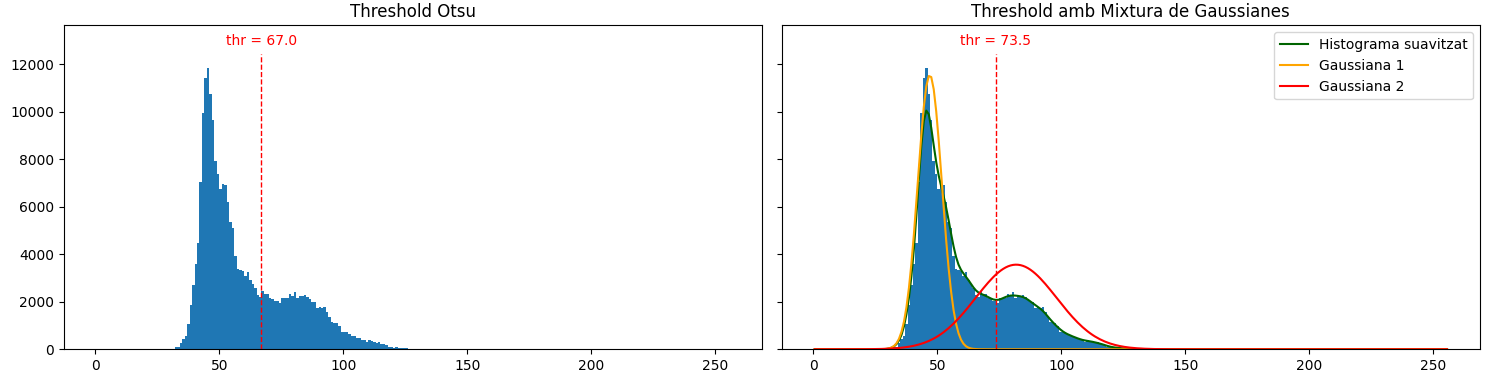
\includegraphics[width=\linewidth]{figs/thresholds}
	\caption{Exemple d'histograma amb els llindars tractats}
	\label{fig:f}
\end{figure}
\\
Així doncs, hem trobat una solució per corregir el llindar que consisteix a fer una \textbf{mixtura de gaussianes} sobre mostres reduïdes de la imatge (per eficiència) i escollir el mínim de l’histograma suavitzat entre els pics de les gaussianes estimades. A la Figura~\ref{fig:f} es poden veure les diferències entre els dos mètodes.

Feta la binarització amb l’últim llindar, l’hem utilitzada per extreure les vores de les barres del pas de zebra. Hem provat dues tècniques: \textbf{Canny} i \textbf{LoG}. Totes dues han donat resultats similars, però hem continuat amb \textbf{LoG} per dues raons: no depèn d’hiperparàmetres com els llindars de Canny, i no fa vores fines, fet que restringeix menys la detecció de línies amb Hough.
\begin{figure}[!h]
	\centering
	\begin{subfigure}{0.31\columnwidth}
		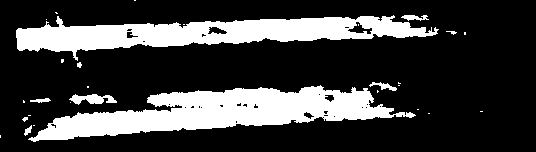
\includegraphics[width=\linewidth]{figs/mog}
		\caption{Imatge binaritzada}
	\end{subfigure}
	\ 
	\begin{subfigure}{0.31\columnwidth}
		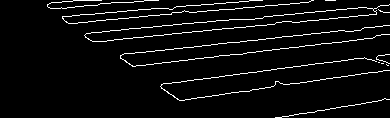
\includegraphics[width=\linewidth]{figs/canny}
		\caption{Canny}
	\end{subfigure}
	\ 
	\begin{subfigure}{0.31\columnwidth}
		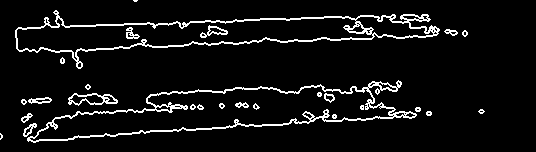
\includegraphics[width=\linewidth]{figs/log}
		\caption{LoG}
	\end{subfigure}
	\caption{Exemple de detecció de vores}
	\label{fig:hough}
\end{figure}
\\
Amb les vores del pas de zebra detectades, només ha faltat extreure les rectes amb \textbf{transformades de Hough}, però aquesta tècnica també depèn d'un llindar. Quan és molt alt no es detecten totes les línies, i quan és molt baix es detecten masses línies errònies. És una tècnica molt sensible a errors, com hem pogut comprovar quan la hem implementat a mà a mode de prova. Per aconseguir millors resultats, hem fet aquest \textbf{mètode propi}:
\vspace*{-0.15em}
\begin{enumerate}[]
	{\small
	\item Apliquem Hough amb llindar alt per obtenir poques línies fiables
	\item Trobem les seves interseccions (punts de fuga)
	\item Agrupem les interseccions properes amb clusterització
	\item Apliquem Hough amb llindar baix per obtenir moltes línies
	\item Eliminem les línies que no es dirigeixen als punts de fuga (errònies)
}
\end{enumerate}

\begin{figure}[!h]
	\centering
	\begin{subfigure}{0.45\columnwidth}
		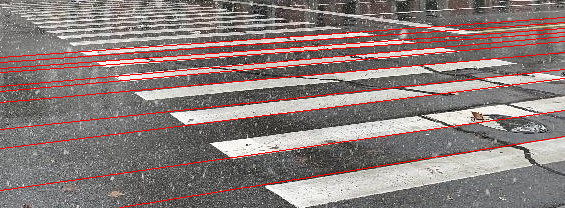
\includegraphics[width=\linewidth]{figs/Hough_restrictiu}
		\caption{Llindar restrictiu}
	\end{subfigure}
	\quad 
	\begin{subfigure}{0.45\columnwidth}
		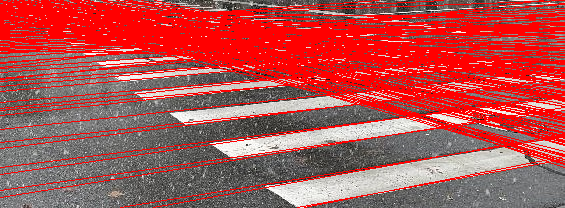
\includegraphics[width=\linewidth]{figs/Hough_molt_tolerant}
		\caption{Llindar molt tolerant}
	\end{subfigure}
	\ 
	\begin{subfigure}{0.45\columnwidth}
		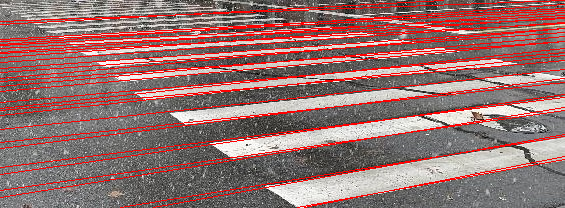
\includegraphics[width=\linewidth]{figs/filtrat_fuga}
		\caption{Filtratge segons punt de fuga}
	\end{subfigure}
	\quad
	\begin{subfigure}{0.45\columnwidth}
		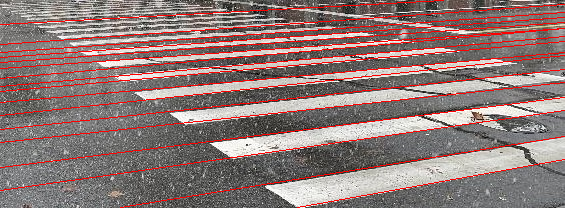
\includegraphics[width=\linewidth]{figs/filtrat_proximitat}
		\caption{Filtratge segons proximitat}
	\end{subfigure}
	\caption{Exemple de filtratge de línies}
	\label{fig:vores}
\end{figure}

Aquest


%\begin{table}[!h]
%\centering
%\begin{tabular}{lccccc}
% x & sin(x) &	cos(x)& tan(x) &  sec(x) & cosec(x)\\
%\hline
%30$^\circ$ & 0.5000 & 0.8660 & 0.5774 & 1.1547 & 2.0000\\
%45$^\circ$ & 0.7071 & 0.7071 & 1.0000 & 1.4142 & 1.4142\\
%60$^\circ$ & 0.8660 & 0.5000 & 1.7321 & 2.0000 & 1.1547\\
%\hline
%\end{tabular}
%\caption{ Raons trigonomètriques per diferents valors d’angles.}
%\label{t:raonstrigonometriques}
%\end{table}


%\section{Conclusions}


\begin{thebibliography}{9}\label{sec:biblio}
	
	\bibitem{YOLO}
	J. Redmon, \textit{\href{https://pjreddie.com/darknet/yolo/}{YOLO: Real-Time Object Detection}}.
	
%	\subsection*{Projectes}
	\bibitem{ImVisible}
	S. Yu et al., \textit{\href{https://github.com/samuelyu2002/ImVisible}{ImVisible: Pedestrian Traffic Light Dataset, LytNet Neural Network, and Mobile Application for the Visually Impaired}}. GitHub repository.
	
	\bibitem{CrosswalksYOLO}
	N. Kuznetsov, \textit{\href{https://github.com/xN1ckuz/Crosswalks-Detection-using-YOLO}{Crosswalks Detection using YOLO: A Supervised Method for Detecting Pedestrian Crosswalks}}. GitHub repository.
	
	\bibitem{CVCPedestrian}
	CVC UAB, \textit{\href{https://www.cvc.uab.es/portfolio/?page_id=3872}{Real-time detection of people and bicycles in pedestrian crossings}}.
	
	\bibitem{PedestrianDetection}
	R. Santos, \textit{\href{https://github.com/ronaldosm/PedestrianTrafficLightsAndCrosswalkDetection}{PedestrianTrafficLightsAndCrosswalkDetection}}. GitHub repository.
	
%	\subsection*{Articles}
	\bibitem{ZebraAI}
	M. A. Rahman et al., \textit{\href{https://www.researchgate.net/publication/354299232_Zebra_Crossing_Detection_and_Time_Scheduling_Accuracy_Enhancement_Optimization_Using_Artificial_Intelligence}{Zebra Crossing Detection and Time Scheduling Accuracy Enhancement Optimization Using Artificial Intelligence}}. ResearchGate, 2021.
	
	\bibitem{ZebraPartiallySighted}
	D. Bradley and A. Dunlop, \textit{\href{https://scispace.com/pdf/zebra-crossing-detection-for-the-partially-sighted-22q9n427id.pdf}{Zebra Crossing Detection for the Partially Sighted}}.
	
	\bibitem{ZebraRecognizer}
	D. Ahmetovic et al., \textit{\href{https://dragan.ahmetovic.it/pdf/ahmetovic2014zebrarecognizer.pdf}{ZebraRecognizer: efficient and precise localization of pedestrian crossings.}}. 2014.
	
	\bibitem{CascadedHough}
	J. Zhang and L. Wang, \textit{\href{https://www.degruyterbrill.com/document/doi/10.1515/comp-2022-0260/html}{Zebra-crossing detection based on cascaded Hough transform principle and vanishing point characteristics}}. De Gruyter, 2022.
	
	\bibitem{ZebraImageProcessing}
	P. Sharma and R. K. Singh, \textit{\href{https://www.ijese.org/wp-content/uploads/Papers/v13i3/B104214020125.pdf}{Zebra Crossing Detection using Image Processing Techniques}}. IJESE, 2022.
	
	\bibitem{RobustPedestrian}
	Y. Chen et al., \textit{\href{https://www.sciencedirect.com/science/article/abs/pii/S0031320316300826}{ZebraRecognizer: Pedestrian crossing recognition for people with visual impairment or blindness}}. Pattern Recognition, 2016.
	
%	\subsection*{Datasets}
	
	\bibitem{RoboflowJuly6}
	Dkdkd. \href{https://universe.roboflow.com/dkdkd/july_6}{\textit{july\_6 Dataset}}. Roboflow Universe, juny 2024.
	
	\bibitem{RoboflowCapstone}
	Dkdkd. \href{https://universe.roboflow.com/dkdkd/capstone-for-detection}{\textit{capstone for detection Dataset}}. Roboflow Universe, juny 2024.
	
	\bibitem{RoboflowAugmented}
	Dkdkd. \href{https://universe.roboflow.com/dkdkd/capstone-for-detection1}{\textit{capstone for detection1 Dataset}}. Roboflow Universe, juny 2024.
	
	\bibitem{RoboflowMultiView}
	Esera. \href{https://universe.roboflow.com/esera/crosswalk-cz3sx}{\textit{crosswalk Dataset}}. Roboflow Universe, agost 2024.
	
	\bibitem{GlobalStreetscapes}
	UALSG. \href{https://github.com/ualsg/global-streetscapes}{\textit{Global Streetscapes Dataset for Crosswalk Detection}}. GitHub repository.
	
	
	
\end{thebibliography}
\end{document}

